\chapter{Approach}
\label{ch:approach}
%As has been discussed in Chapter \ref{ch:related}, there is a need for a tool which can detect all the encountered syntax errors in RDF documents to ensure their quality and to make RDF diagnostics easy for users instead of showing only the first detected syntax error, struggling them in finding the other syntax errors if exist. 
In this chapter, we present RDF-Doctor, an approach towards realization of a comprehensive parser for syntax validation and recovery.
RDF-Doctor is able to identify more than one syntax error at the same time and provide meaningful messages.
%order to fill this need, this study was held to propose a proper solution. 
Then, main components of RDF-Doctor are discussed in detail along with possibilities of integration serialization formats, such as Turtle and N-Triple. Finally, this chapter ends with presenting the categories of syntax errors.


\section{Overview of RDF-Doctor Approach}

This section covers the core component of the approach, then discusses the main processing steps, and ends with elaborating the categories of RDF syntax errors to ease the road to the appropriate solution. 

\subsection{ANTLR: The Core Component}

The core component inside RDF-Doctor is the ANTLR framework. It is used to automatically generate a parser based our developed grammar, including predefined error production rules to match sequences of tokens that contains RDF syntax errors.
%In order to find a parser which can accept the error production rules in its grammar, our choice was to use ANTLR framework to automatically generate the required parser.
%Equally important lots of handy features in ANTLR motivate its usage in the proposed solution to generate the internal parser, and also as an imported library for compiling and  running  of RDF-Doctor. 
The ANTLR framework has several important features: 1) a given grammar can equip with error production rules and when a couple of tokens match such rules, the parser will fire an error notification; 2) it uses a parse tree to parse input tokens and the view of this parse tree can be delivered as one of the outputs to the user at the end of parsing process; and 3)it supports the auto-generation of parsers in different programming languages.
%which is an one-to-many added value, where one grammar file can automatically generate of the programming languages.

%\begin{itemize}
% \item \textbf {Input}: It is the role of the user to provide an RDF file with certain options, such as 1) enabling/disabling of the error correction; 2) showing an error report of JSON\footnote{https://www.json.org/} or text format; and 3) concealing/showing up the parse tree.


%\item \textbf{Processing}: starts with preparing the input to be parsed in the following workflow: 1)it reads the input; 2) splits it into smaller pieces if needed; 3) parses the input for each slice (if many); and 4) corrects a subset of detected syntax errors. 
%This phase utilizes the parser built based on a predefined grammar.
%it requires ANTLR library for parsing, and some options from the user to activate/deactive some features of the solution.   
%\item \textbf{Output}: provides the reports after processing phase, %including 1) an error report to announce the detected syntax errors; 2) a correction report which lists the recovered syntax errors; and 3) an output file after healing some of the detected syntax errors\todo{It is not clear what is the point number 3}; and 4) a frame contains the parse tree. 
%Both, the correction report and the output file require to be enabled in order to be generated. 
%\end{itemize}


\subsection{Main Processing Steps}

\begin{figure}
	\centering
	  	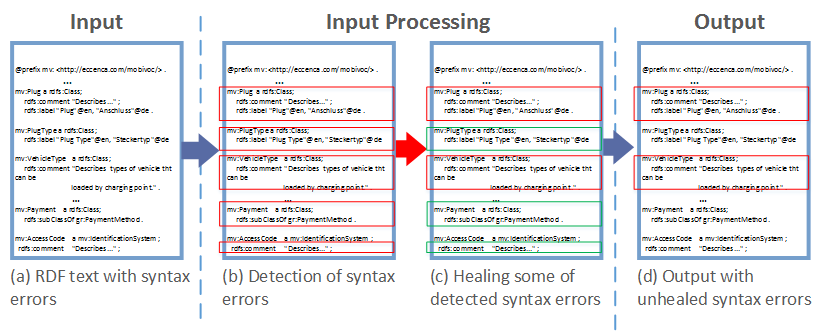
\includegraphics[width=1\textwidth]{images/Approach.png}
		\caption{\textbf{RDF-Doctor workflow.} The user writes or edits his own RDF file, then sends it to RDF-Doctor for parsing.
		Next, RDF-Doctor can divide the input in multiple chucks, in the case of a large input, or use the same input file. 
		Each input chunk or file is parsed to detect any syntax errors if they exist, then it recovers a subset of detected errors, if the automatic error recovery feature is enabled by the user. 
		Finally, RDF-Doctor outputs a parse tree, a correction report, an error report, and an output file, including an RDF file after error recovery.}
		\label{Fig:Approach}  
\end{figure}

The workflow of RDF-Doctor illustrated in Figure \ref{Fig:Approach} and its architecture depicted in Figure \ref{Fig:Architecture} are discussed in the significant steps of RDF-Doctor in the following:
%shows the technique used to handle an RDF text, including a couple of  syntax errors. 
%In the following, the main milestones of this approach are explained in 4 sequential steps:

 \begin{enumerate}[label=(\alph*)]
\item \textbf{Reading RDF files}: An ordinary RDF file is submitted to RDF-Doctor, this is the Input phase, as described in Figure~\ref{Fig:Approach} (a).
Initially, Processing components in Figure \ref{Fig:Architecture} read the submitted file. In the case that the file is too large (more than 1 million triples), then it is segmented into two or more chunks based on the number of triples. 
Each chunk is parsed and processed separately from others in this step.
%%%%%%%%%%%%%%%%%%%%
Moreover, certain options can be selected by the user before submitting the file, such as 1) enabling/disabling of the automatic error correction; 2) showing an error report in either  JSON~\footnote{\url{https://www.json.org/}} or text format; and 3) concealing/showing up the parse tree diagram at the end of parsing process.
%%%%%%%%%%%%%%%%%%%%
%{Figure \ref{Fig:Approach}}(a) simulates the actual work of this step where a submission of an RDF file with syntax errors is assumed. 
\item \textbf{Detecting of syntax errors}: Parsing is the third step in  the Process phase in Figure \ref{Fig:Architecture}, in which the parser has predefined rules for syntax errors,  %(these rules are titled with error production rules, presented in Error Recovery Methodologies in Chapter \ref{ch:preliminaries}), 
\begin{figure}[ht]
	\begin{center}
		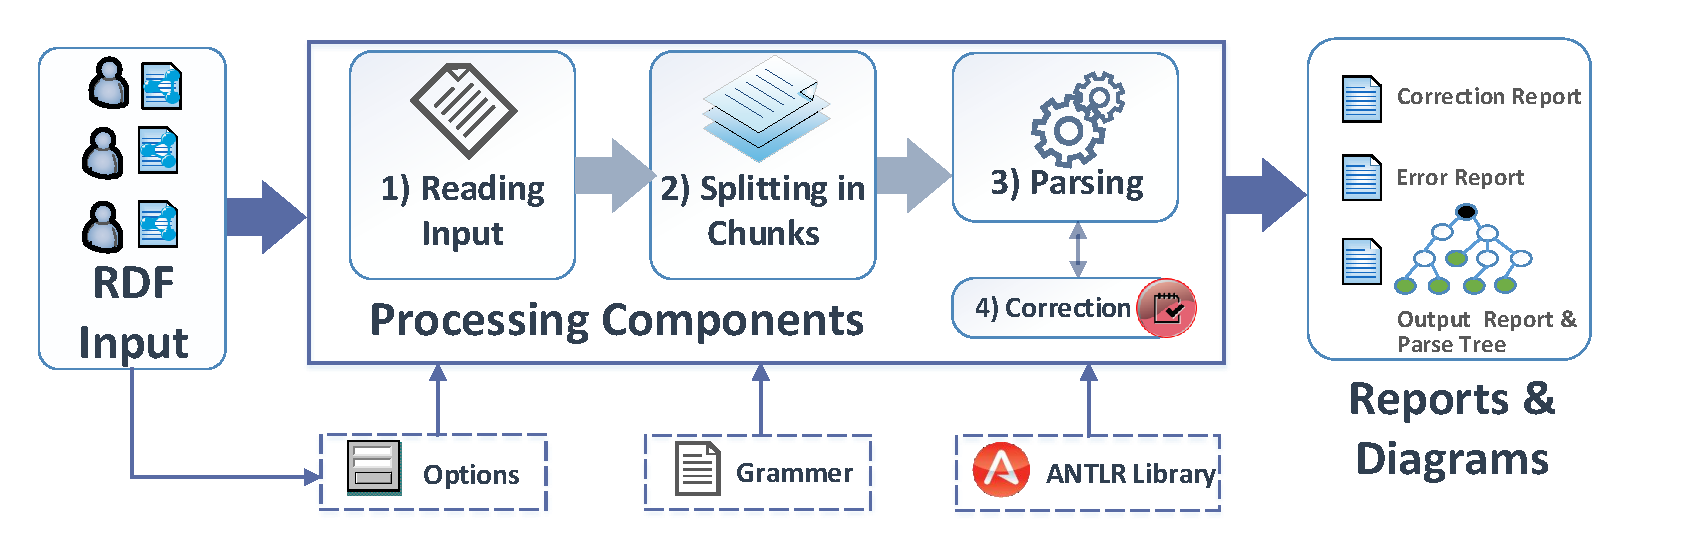
\includegraphics[scale=0.5]{images/architecture.pdf}
	\caption{\textbf{RDF-Doctor architecture.} It consists of Input, Processing, and Output phases. 
		In the Input phase, users send their RDF data. The Processing phase reads the data, splits them into smaller chunks if they are large, then continues parsing and recovery of certain errors.
		In this phase, a user action is required to enable/disable the error recovery.
	    Finally, the Output phase presents reports for error detection and recovered error, as well as a parse tree.}
		\label{Fig:Architecture}
	\end{center}
\end{figure}
once a rule is matched with a sequence of input tokens, it raises a flag to the error listener API which later is listed in the final error report. 
Reading of input tokens continues until the end of the file while searching for any match in order to identify potential syntax errors. 
In {Figure \ref{Fig:Approach}}(b) lines surrounded with \emph{red color} depict the detected lines which contain syntax errors.
%%%%%%%%%%%%%%%%%%%%%%%
%%%%%%%%%%%%%%%%%%%%%%%
To have a deep thought on the internal works of the parser to detect syntax errors using a parse tree. Figure \ref{Fig:approachParseTree} shows how each sub-tree of the root node (acts as the starting rule) is a rule containing either a correct syntax or an incorrect one. Each rule is represented by a sub-tree being empty or one and more non-terminals (considered as rules in the grammar) and one and more terminals (they are lexical forms of input tokens). A sub-tree produces an syntax error, if all of its terminals (shown in \emph{red color} in Figure \ref{Fig:approachParseTree}) formulate an error production rule of grammar rules. Hence in both sub-trees 2\textsuperscript{nd} and 4\textsuperscript{th} from left-to-right over Figure \ref{Fig:approachParseTree} are rules with a sequence of tokens producing syntax errors.  Meanwhile other sub-tree 1\textsuperscript{st},  3\textsuperscript{rd}, and 5\textsuperscript{th} with terminals in \emph{green color}  are including  correct syntactic  forms.


\item \textbf {Healing a subset of encountered syntax errors}:%%%%%%%%%%%%%%%%%%%%
 { Figure} \ref{Fig:Architecture} shows this feature as the  4\textsuperscript{th} of processing components. %%%%%%%%%%%%%%%%%%%%
Firstly, it needs to be manually activated by the user, since it is disabled by default. Secondly, the method of syntax error recovery currently focuses on a certain type of errors which has only one predefined solution to correct them. Examples of such errors are  missing  a dot at the end of a triple, missing a semi-colon after multiple predicates sharing same subject, or missing a comma after multiple objects having same subject and predicate. Lines surrounded with \emph{green color} in {Figure~\ref{Fig:Approach}}(c) represent some of the healed lines from error at the end of the correction phase. 

\item\textbf {Producing of the output}: The output phase, demonstrated in Figure \ref{Fig:Architecture}, assumed the activation of automatic correction feature by the user. Additionally, {Figure \ref{Fig:Approach}}(d) describes how the output file looks like at the end of this phase.    It shows lines containing errors are already recovered, whereas other lines still are unhealed. Commonly, errors that cannot be recovered by RDF-Doctor without user intervention, are those errors which can have several solutions, for example, a literal with multiple language tags like ``me"@en@de which shows a string with two language tags and since the solution would be an omission of one of them but the intention of the user is unknown in this sense. In addition, there exist errors with undefined or unknown recovery solution, for example, missing of a user-defined prefix declaration for a certain local namespace which cannot be guessed since it is only known by the user himself. 
\end{enumerate} 
\begin{figure}
	\centering
	  	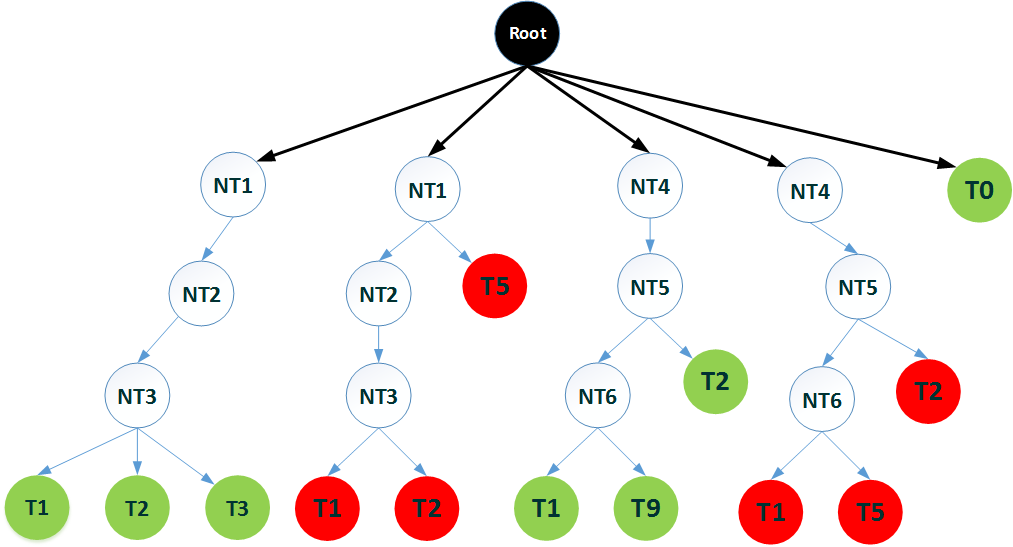
\includegraphics[width=.8\textwidth]{images/approachParseTree.png}
		\caption{\textbf{Detection of syntax errors while traversing the parse tree.} 
		Root node is the head of the first rule in the grammar and the head of the parse tree.
		All the children of the root are either non-terminal nodes represented by ``NT" followed by an number or  terminal ones shown by ``T" succeeded by a number. 
		A syntax error can be detected on a non-terminal node when all of its terminals represent a sequence of tokens that is a statement including a syntax error. Red terminals represent error-inclusive statements and green ones represent error-free statements.}
		\label{Fig:approachParseTree}  
\end{figure}


To functionally represent the approach of this study, Algorithm \ref{alg:algorithm-main} was engineered. 
It shows the abstract behaviour of RDF-Doctor where \textbf{syntaxRules} variable combines both correct syntax rules and incorrect ones. 
A \textbf{while loop} carries on until reaching the current end of file or chunk, if a large file is separated into several chunks. 
The \textbf{ruleToBeMatched} variable incloses one rule of either correct or incorrect production rules, formed by the supplied tokens. While the variable \textbf{currentTokens} stores a sequence of current supplied tokens to check to which rule, it belongs.  

Since the crucial step is to find encountered syntax errors, \textbf{ruleToBeMatched} is evaluated to check if its content is matched any of \textbf{incorrectSyntaxRules}. If this the case, then the content of \textbf{currentTokens} is considered as a syntax error, and the parser sends an error notification to any subscribed error listener API, in order to further process of the collected errors. 

\begin{algorithm}[] 
 \caption{The pseudo-code of RDF-Doctor}
 \label{alg:algorithm-main}
 \KwData{inputText, correctSyntaxRules, incorrectSyntaxRules, CorrectionIsSelected}
 \KwResult{foundSyntaxErrors and recoveredSyntaxErrors}
% S = subject(M)\;
foundSyntaxErrors = [ ];\\
recoveredSyntaxErrors = [ ];\\
$syntaxRules \leftarrow correctSyntaxRules + incorrectSyntaxRules;$\\
		\While{token in inputText \&\& $inputText \neq EOF$}{
		currentTokens += token;\\
ruleToBeMatched += lex(token);\\
		\uIf{ syntaxRules contains ruleToBeMatched}{
		\uIf{ incorrectSyntaxRules contains ruleToBeMatched}{
		 foundSyntaxErrors.push(currentTokens);\\
		\uIf{ CorrectionIsSelected}{
		\uIf{ canErrorRecovered(ruleToBeMatched)}{
		  \uIf{recoverSyntaxError(currentTokens)}{
		  recoveredSyntaxErrors.push(currentTokens);\\
		  foundSyntaxErrors.pop(currentTokens);\\

		  }
		}
		}
		}
		 $currentTokens \leftarrow ""$  \\
		 $ruleToBeMatched \leftarrow ""$  \\
		 $token \leftarrow ""$  	\\	
		}
}
return foundSyntaxErrors , recoveredSyntaxErrors
\end{algorithm}

The automatic correction of errors is a feature that can be activated as an additional option when running RDF-Doctor. 
In the case that the user selects to enable it, then the \emph{Error Correction Module} will traverse the entire list of detected syntax errors and based on the error message, it can identify if the error can be unquestionably corrected or needs a user intervention. 
At the end of the correction phase, a report of the corrected errors will be delivered to the user. 

\section{Categories of RDF Syntax Errors}

In this approach, Turtle and N-Triples RDF serializations are used as the use case syntaxes. 
Hence, Turtle is a special case of N-Triples. For this reason, the grammar of RDF-Doctor was created based on Turtle serialization. 
Furthermore, since the significant part in this study is the ability to identify syntax errors, the expected syntax errors need to be known in advance in order to be injected in the grammar. 
A suite of Turtle syntax errors are presented in ~\cite{TurtleTests:Online} plays an important role in syntax errors declaration. It contains several files in Turtle with an objective of showing both correct and incorrect syntaxes. Additionally, a filename in~\cite{TurtleTests:Online}, i.e., if it contains the word ``Bad", it means that it contains an incorrect syntax, which can be syntactically engineered in our grammar.

 \begin{table*}[tbp]
 	\centering
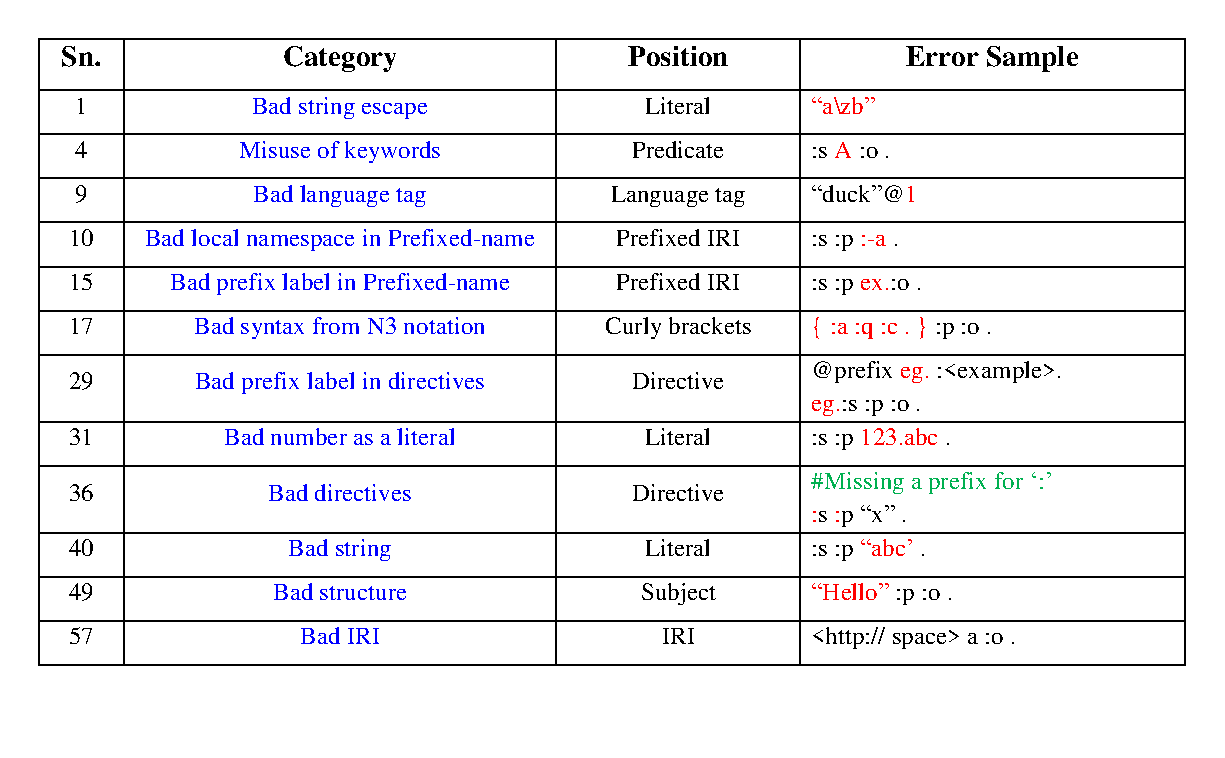
\includegraphics[width=5.5in]{images/TrimmedBigTable.pdf}
		\setlength\abovecaptionskip{-10mm}
	\caption{\textbf{Categories of a subset of syntax errors of N-Triple and Turtle serializations}.
	This table is a part of Appendix~\ref{tab:syntaxErrorCate} which shows one sample of each category. The serial numbers take the same order of rows in the referred table. 
	Position represents a term related to Turtle and N-Triple serializations where the actual syntax error is located.}
	\label{tab:trimmedTable}
\end{table*}


In table \ref{tab:trimmedTable}, we have categorized types of syntax errors into multiple categories. These categories are taking from the filenames in~\cite{TurtleTests:Online} with some modification to become meaningful. The table shows each category with one error sample and an error position where the actual syntax error is located. Indeed, this helps much in designing of the grammar rules and also to identify which of them can be automatically corrected. Details including more samples of these categories are provided in Appendix~\ref{tab:syntaxErrorCate}.     
